\subsubsection*{The following algorithms have been considered to solve the jewel problem}
As mentioned the two things that can potentially hope to minimize the search time needed to solve a sokoban problem, namely a 'good' heuristic search and search tree pruning. The search algorithm, and therefore by extension also the heuristic function, is concerned with the 'get next state in search tree' part of the algorithm in listing \ref{code:sokoalgo}, and pruning is concerned with the 'is state valid' part.

\subsubsection*{A*}
This was the first algorithm considered using for the problem, because it is both optimal, complete and fast if a good heuristic function is used.
It has however proven fairly difficult to find a 'good' admissible heuristic for the jewel problem. One of the only possibilities that have come to mind is the sum of each jewels manhatten distance to it's closest goal. This heuristic would be admissible, since the closest distance from a jewel to a goal would naturally be the minimum amount of moves needed to move the jewel in order to solve the problem. It is our assessment that this heuristic unfortunately can not be characterized as a very good one, since the sum of smallest distances between jewels and goals, is by no means an estimate of the number of moves left to solve the problem, due to the intrinsic complexity of most sokoban problems (jewels getting in the way of other jewels, jewels being blocked by walls etc.). In other words, a good A* heuristic should guide the search down the branch of the search tree most likely to contain an acceptable solution, thereby minimizing the nodes/states that would have to be traversed in order to get to a solution. The considered heuristic would not necessarily be able to do so.
The cost that would be used in this implementation, would be the total number of moves the robot/man would have to take to move the jewel to the desired position plus the robot moves taken to get from the initial state (root state) to the current state.

\subsubsection*{Greedy search}
By disregarding the Heuristic function from the A* search, and instead using the cost of robot movements as the heuristic, we would in effect get a greedy search. We would use a so called closed list, to avoid loops, thereby attaining completeness. The downside of this algorithm however is that it is not optimal, which is a requirement if we are to get a solution with the minimum required number of robot movements.

\subsubsection*{Breadth first search}
The breadth first search algorithm is inherently slow for complex problems, but is however optimal in so called unit-step cases (the cost from one state to the next is always the same), which speaks greatly in favour of this algorithm in this case. However for this to work it is important to remember that the unit-step requirements necessitates an implementation where each robot movement spawns a new state, as opposed to just spawning a new state for each jewel movement, so that the depth of the solution in the tree will correspond with the number of movements performed by the robot. The use of this algorithm therefore requires that the two subproblems be solved as one. This will, among other things, increase the amount of memory needed by the algorithm. 

\subsubsection*{Uniform cost search}
A variation on the breadth first search and greedy search exists, where the next node visited is the one with the least total cost from the root node (the same cost as used in the A* algorithm), as opposed to the greedy search where the next state visited is the one with the least cost from the current node, which was the cause of the non optimality of the greedy search. This is therefore both a complete and optimal algorithm in terms of minimum robot movements, when using the robot movements as cost. Furthermore it does not require, as the breadth first search, that the sokoban problem not be solved as two subproblems.

\subsubsection*{Search tree pruning}
Since a good heuristic function has not been found for the search algorithm, the time complexity of the solver will presumably be high, unless the search tree can be pruned significantly. Fortunately the sokoban problem is one where a large amount of pruning is possible in terms of deadlock detection. 

\begin{figure}[ht]
\centering
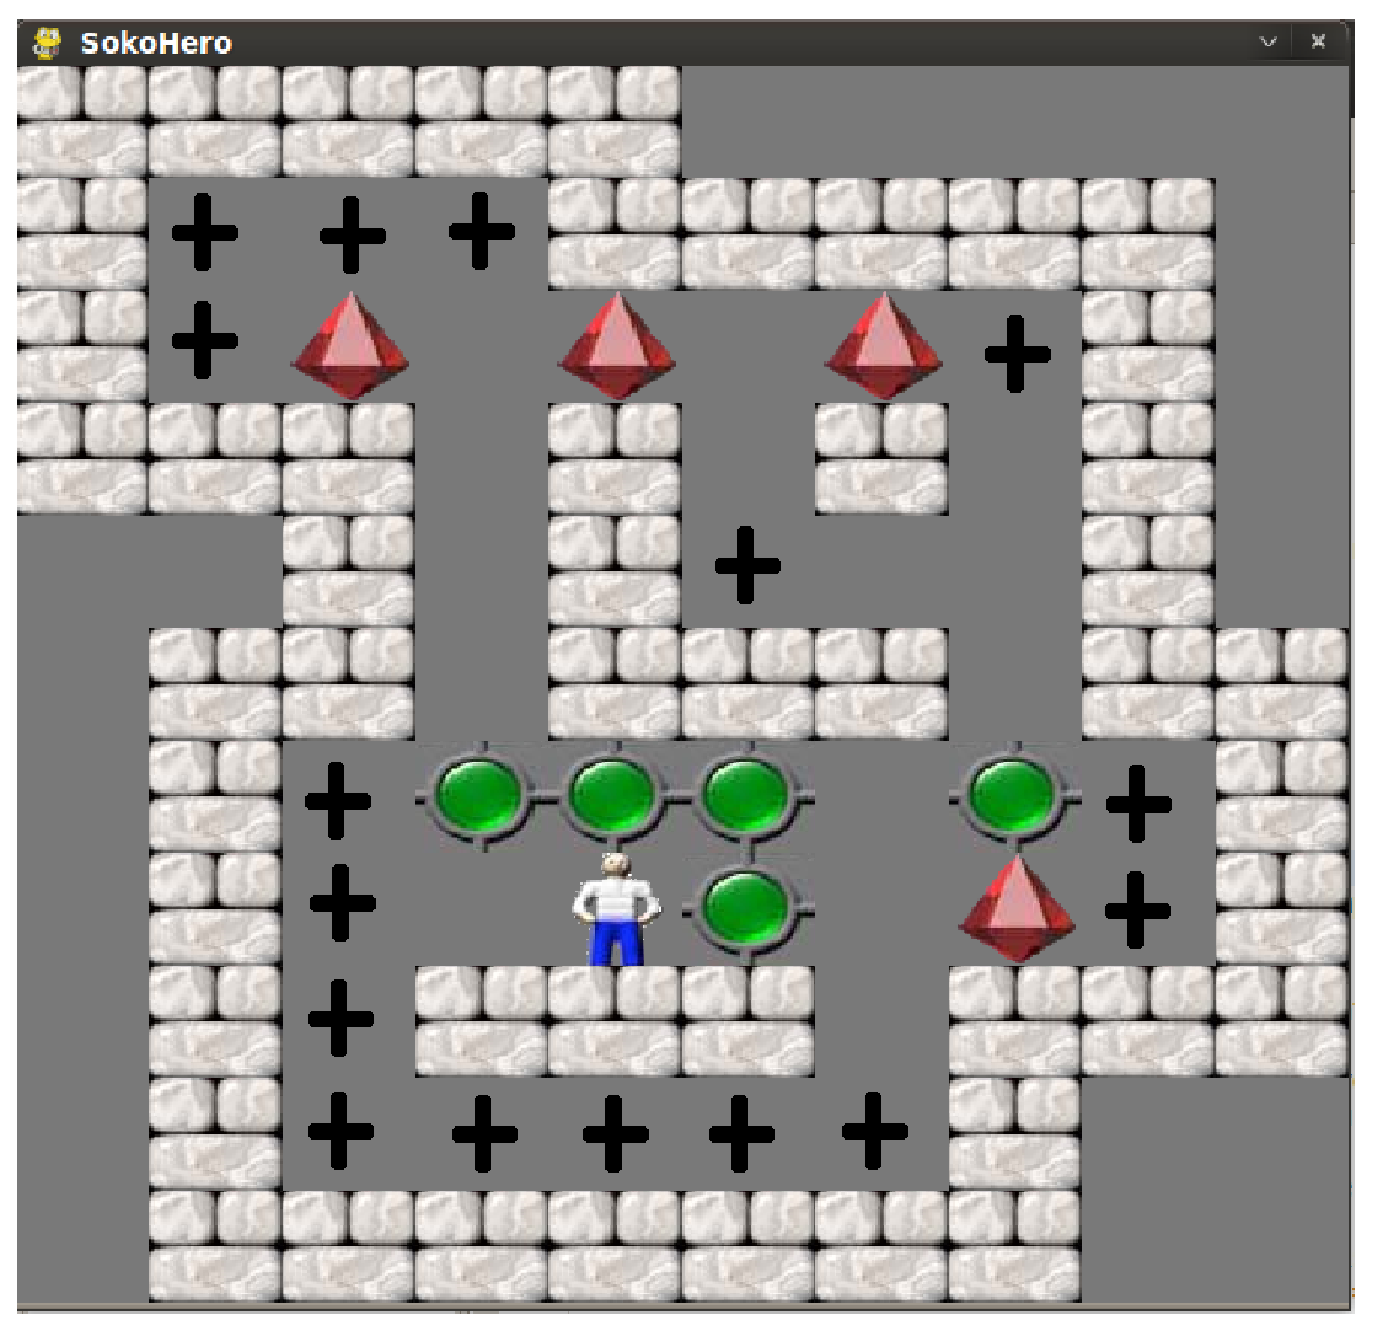
\includegraphics[scale=0.25]{images/sokohero_deadlocks.eps}
\caption{A screenshot of a sokoban game with deadlock zones marked with '+'}
\label{fig:sokoherodeadlocks}
\end{figure}

Figure \ref{fig:sokoherodeadlocks} shows all the zones where the placement of a jewel would result in an unsolvable problem, meaning that the state and all states spawned from that one are useless, and would only potentially waste the time of the solver if it would have to visit them.
\\
The following deadlock detection algorithm is devised, where return true symbolises that the state has a deadlock:

\begin{lstlisting}[language=Ruby, frame=single, basicstyle=\scriptsize, caption={Deadlock detection pseudo code}, label={code:deaddetect}]
For each jewel do:
  if jewel in corner:
    return true
  if jewel against vertical wall:
    for each square above jewel:
      if square is goal:
        return false
      if square on the obstructed side of jewel is empty or goal or jewel:
        return false
    for each square below jewel:
      if square is goal:
        return false
      if square on the obstructed side of jewel is empty or goal or jewel:
        return false
  if jewel against horizontal wall:
    for each square to the right of jewel:
      if square is goal:
        return false
      if square on the obstructed side of jewel is empty or goal or jewel:
        return false
    for each square to the left of jewel:
      if square is goal:
        return false
      if square on the obstructed side of jewel is empty or goal or jewel:
        return false
  return true
\end{lstlisting}

This deadlock detection algorithm could be improved further by checking for deadlocks due to one jewel obstructing another in a irreversible way. Due to the deadline of the project however, it has not been possible to include this feature.

\subsubsection*{The following algorithms have been considered to solve the path finding problem}
\subsubsection*{A*}
This algorithm is very often used as path finding algorithms in games, because good heuristic functions are relatively easy to find when confronted with such problems. Often the manhatten distance to the goal is sufficient enough to give very fast searches compared to depth- or breadth first. Therefore we do not consider any other searches for the path finding problem.

\subsection{Choosing the search algorithm}
Naturally the A* algorithm will be used to solve the path finding problem. The choice of search algorithm for the jewel problem would have fallen on the Uniform Cost Search algorithm, because it gives an optimal solution in terms of robot movements which is of most importance, since the time to solve the problem is irrelevant because the specific problem as mentioned will be given a week in advance. We will however, out of pure academical interest, implement all of the considered algorithms for the jewel problem, in order to compare their performances. 
